\documentclass[12pt]{report}
% Preamble: Contains packages and user-defined commands and settings
\usepackage{amsmath,amsxtra,amssymb,latexsym, amscd,amsthm}
\usepackage{color,indentfirst}
\usepackage[utf8]{vietnam}
\usepackage[left=30mm,right=20mm,top=30mm,bottom=35mm]{geometry}
\usepackage{fancyhdr}

%\usepackage{amsfonts}
\usepackage{longtable}
\usepackage{pgf,tikz}
%\usepackage{mathrsfs}
\usetikzlibrary{arrows}
\usepackage{enumerate}
\pagenumbering{arabic}
\usepackage{enumerate}
\usepackage{cases}
\usepackage{verbatim}
\usepackage{rotating}
\usepackage{wrapfig}
\usepackage{setspace}
\usepackage{subcaption}
%\singlespacing
\onehalfspacing
%\doublespacing
%\setstretch{1.1}
% \usepackage{xypic,tikz}
% \usepackage{tikz-cd}
\usepackage[colorlinks=true, linkcolor=blue]{hyperref}
% \usepackage{setspace}

% \usepackage[unicode,pdfborder={0 0 0},colorlinks=true, linkcolor=blue]{hyperref}

\renewcommand{\theequation}{\arabic{chapter}.\arabic{section}.\arabic{equation}}

\newtheorem{thm}{Theorem}[section]

\newtheorem{corollary}{\bf Hệ quả}[section]


\theoremstyle{definition}
\newtheorem{definition}[thm]{\bf Định nghĩa}
\newcommand{\dn}{\begin{definition}}
\newcommand{\hdn}{\end{definition}}


\newtheorem{example}[thm]{\bf Ví dụ}
\newcommand{\vd}{\begin{example}}
\newcommand{\hvd}{\end{example}}


\theoremstyle{proposition}
\newtheorem{proposition}[thm]{\bf Mệnh đề}
\newcommand{\md}{\begin{proposition}}
\newcommand{\hmd}{\end{proposition}}



\newtheorem{remark}[thm]{\bf Hệ quả}
\newcommand{\hq}{\begin{remark}}
\newcommand{\hhq}{\end{remark}}



\newtheorem{lemma}[thm]{\bf Bổ đề}
\newcommand{\bd}{\begin{lemma}}
\newcommand{\hbd}{\end{lemma}}

\newtheorem{algorithm}[thm]{\bf Thuật toán}
\newcommand{\alo}{\begin{algorithm}}
\newcommand{\ealo}{\end{algorithm}}




\newtheorem{theorem}[thm]{\bf Định lý}
\newcommand{\dl}{\begin{theorem}}
\newcommand{\hdl}{\end{theorem}}

\theoremstyle{break} 
%\theorembodyfont{\normalfont} 


\usepackage{enumerate}
\usepackage{graphicx}
\newcommand{\Rn}{ \mathbb{R}^n }
\newcommand{\Zn}{ \mathbb{Z}^n }
\newcommand{\Rns}{ (\mathbb{R}^n)^* }



\newcommand{\Ndn}{ \overset{\vee }{\sigma}}
\newcommand{\tdn}{ \overset{\vee }{\tau}}

\DeclareMathOperator\Conv{Conv}
\DeclareMathOperator\codim{codim}

%------------------------------------------dinh dang moi truong---------------------------------------------------------------------------------------%
\makeindex

\setcounter{secnumdepth}{3} %tao so cho subsubsection
%+ Bat dau tai lieu tai day.

\def\N{\mathbb{N}}
\def\Z{\mathbb{Z}}
\def\R{\mathbb{R}}
\def\Q{\mathbb{Q}}
\def\C{\mathbb{C}}  
\def\K{\mathbb{K}}  
\def\F{\mathbb{F}}  
\def\L{\mathbb{L}}  
\def\X{\mathbb{X}}

\begin{document}
\begin{titlepage}
\fontsize{14pt}{23pt}\selectfont
\newpage
\thispagestyle{empty}%không đánh số trang,không tiêu đề, "roman=số la mã i, ii, iv,$\ldots$ ", "arabic=1,2,3,$\ldots$ "
%\setcounter{page}{0}%đặt lại số trang bắt đầu từ 0

\begin{center}
\large\textbf{ ĐẠI HỌC QUỐC GIA TP. HỒ CHÍ MINH} \\
\large \textbf{TRƯỜNG ĐẠI HỌC KHOA HỌC TỰ NHIÊN} \\


\vspace*{2.5cm}

{\bf \large LƯU QUANG NHIÊN}
\vspace*{4cm}

\begin{center}
\Large{\textbf{BAYSIAN CONVOLUTION NEURAL NETWORK}}\\
\end{center}

\vspace*{3cm}

\begin{center}
\bf \large LUẬN VĂN THẠC SĨ TOÁN HỌC\\
\end{center}

\vfill

{\large\bf Hồ Chí Minh - 2019}
\end{center}
\newpage
\thispagestyle{empty}
\begin{center}
\large\textbf{ ĐẠI HỌC QUỐC GIA TP. HỒ CHÍ MINH} \\
\large \textbf{TRƯỜNG ĐẠI HỌC KHOA HỌC TỰ NHIÊN} \\

\vspace*{2.5cm}

{\bf \large LƯU QUANG NHIÊN }
\vspace*{4cm}

\begin{center}
\Large{\textbf{BAYSIAN CONVOLUTION NEURAL NETWORK}}\\
\end{center}

\vspace*{2cm}

\begin{tabular}{l  l }
\large Chuyên ngành&\bf \large: \quad CHUYÊN NGÀNH XÁC SUẤT THỐNG KÊ\\ 
\large Mã ngành&\bf \large: \quad 60460106 \\
\large Mã học viên&\bf \large: \quad 16C23010 \\
\end{tabular}
\vspace*{2cm}

\begin{tabular}{l l }
\bf \large Người hướng dẫn 1&\bf \large:\quad TS.DƯƠNG ĐẶNG XUÂN THÀNH\\[4pt]
\bf \large Người hướng dẫn 2&\bf \large:\quad TS. Mai Hoàng Bảo Ân\\[4pt]

\end{tabular}
\vfill

{\large\bf Hồ Chí Minh - 2019}
\end{center}


\end{titlepage}
\chapter*{\begin{center}Lời cảm ơn\end{center}}
\addcontentsline{toc}{chapter}{Lời cảm ơn} 
\begin{spacing}{1.5}
	
	Tôi xin được bày tỏ lòng biết ơn chân thành và sự kính trọng sâu sắc đến Tiến sĩ Dương Đặng Xuân Thành, Tiến sĩ Mai Hoàng Bảo Ân, hai thầy đã trực tiếp giảng dạy, hướng dẫn và tạo mọi điều kiện trong quá trình học tập và nghiên cứu để tôi có thể hoàn thành luận văn này một cách tốt nhất. 
	Tôi xin chân thành cảm ơn Ban giám hiệu, Phòng Đào tạo sau đại học, Khoa xác suất và thống kê cùng quý thầy cô giáo đã trực tiếp giảng dạy, giúp đỡ tôi trong quá trình học tập tại trường.
	Mặc dù rất cố gắng nhưng do hạn chế  về thời gian, trình độ và kinh nghiệm nghiên cứu nên bên
	cạnh những kết quả đã đạt được, luận văn không thể tránh khỏi những hạn chế và thiếu sót.
	Tôi rất mong nhận được sự góp ý của quý thầy cô và các bạn đồng nghiệp để luận văn được hoàn thiện hơn.
	
\end{spacing}
%\mainmatter
\tableofcontents
\listoffigures
\listoftables
\chapter{Giới thiệu}  %Title of the First Chapter

\ifpdf
    \graphicspath{{Chapter1/Figs/Raster/}{Chapter1/Figs/PDF/}{Chapter1/Figs/}}
\else
    \graphicspath{{Chapter1/Figs/Vector/}{Chapter1/Figs/}}
\fi


%********************************** %First Section  **************************************

Những năm gần đây, AI-Artifical Intelligence (Trí tuệ nhân tạo), và cụ thể hơn là Machine Learning (Học máy) nổi lên như một bằng chứng của cuộc cách mạng công nghiệp lần thứ tư. Trí tuệ nhân tạo len lỏi vào mọi lĩnh vực trong cuộc sống mà có thể chúng ta không nhận ra. Xe tự lái, hệ thống tự tag khuôn mặt trong ảnh của Facebook, trợ lý ảo Siri của Apple, hệ thống gợi ý sản phẩm trên các trang buôn bán điện tử, ... chỉ là một vài trong vô vàn ứng dụng của AI/Machine Learning.\\
Machine Learning(Học máy) là một tập con của AI, nó có khả năng tự học hỏi dựa trên những dữ liệu từ lịch sử mà không cần phải lập trình cụ thể. Những năm gần đây, khi mà khả năng tính toán của máy tính được nâng lên tầm cao mới và bộ dữ liệu khổng lồ được thu tập từ các hãng công nghệ mới, Machine Learning đã tiến thêm một bước dài và lĩnh vực mới ra đời gọi là Deep Learning (Học sâu). Deep Learning đã giúp máy tính thực hiện những việc tưởng chừng không thể như phân loại cả ngàn vật thể khác nhau trong một bức ảnh, tự tạo chú thích cho ảnh, chuẩn đoán bệnh thông qua hình ảnh, giao tiếp với con người. Convolutional neural network (CNNs: Mạng thần kinh tích chập) là một biến thể của Deep Neural Network (DNNs: Mạng thần kinh sâu) đã đạt được độ chính xác vượt con người trong nhiệm vụ phân loại ảnh.\\
Cùng với sự đa dạng của dữ liệu phi tuyến tính, xu hướng các NN hiện nay là càng ngày sâu, càng chồng nhiều lớp với nhau để có thể mô hình hóa được những đặc trưng tốt nhất của dữ liệu. Vì vậy, số lượng tham số hay thể tích của mô hình ngày càng lớn khiến chúng phải cần một khối lượng dữ liệu đào tạo lớn để tránh tình trạng overfitting. Khối lượng lớn ở đây ngoài số lượng còn muốn nói đến sự đa dạng, tổng quát trong dữ liệu và việc bao nhiêu là đủ lớn rất khó để xác định được. Vì vậy, việc mô hình bị overfitting hay không khó để kiểm soát. Cùng với đó, những mô hình NN hiện tại không có khả năng ước lượng độ không chắc chắn của dự đoán của chúng dẫn đến việc quá tự tin quyết định, đưa ra những dự đoán.\\
Trong luận văn này, tôi sẽ giới thiệu về Baysians Neural Network hay cụ thể hơn là Bayesian Convolutional Neural Network (BayesCNN), thay vì tìm một bộ trọng số tối ưu, BayesCNN ước lượng mỗi trong số một phân phối cụ thể giúp mô hình trở nên tổng quát hơn. BayesCNN không chỉ đạt hiệu suất tương đương mà còn đưa ra một ước lượng về độ không chắc chắn cho từng dự đoán, giúp việc quyết định việc có nên tin vào kết quả dự đoán đó của mô hình hay không?\\
\textbf{Nội dung luận văn gồm 6 chương:}\\
	\textit{Chương 1:} Giới thiệu.\\
	\textit{Chương 2:} Kiến thức chuẩn bị.\\
	\textit{Chương 3:} Suy luận Baysian\\
	\textit{Chương 4:} Bayesian Convolutional Neural Networks\\
	\textit{Chương 5:} Ứng dụng vào bài toán phân loại.\\
	\textit{Chương 6:} Kết luận và triển vọng.\\
% !TeX spellcheck = en_US

%!TEX root = ../thesis.tex
%*******************************************************************************
%****************************** Second Chapter *********************************
%*******************************************************************************

\newcommand{\ba}{\mathbf{a}}
\newcommand{\bb}{\mathbf{b}}
%\newcommand{\bd}{\mathbf{d}}
\newcommand{\bw}{\mathbf{w}}
\newcommand{\bx}{\mathbf{x}}
\newcommand{\by}{\mathbf{y}}
\newcommand{\Exp}[2]{\mathbb{E}_{#1}\left[#2\right]}
\newcommand{\Var}[2]{\text{Var}_{#1}\left[#2\right]}
\newcommand{\Cov}[2]{\text{Cov}_{#1}\left[#2\right]}
\newcommand{\Corr}[2]{\text{Corr}_{#1}\left[#2\right]}

\newcommand{\bA}{\mathbf{A}}
\newcommand{\bB}{\mathbf{B}}
\newcommand{\bV}{\mathbf{V}}
\newcommand{\bW}{\mathbf{W}}
\newcommand{\bv}{\mathbf{v}}

\newcommand{\bphi}{\mathbf{\phi}}
\newcommand{\bt}{\mathbf{\theta}}
\newcommand{\bdelta}{\mathbf{\delta}}
\newcommand{\beps}{\mathbf{\epsilon}}
\newcommand{\q}{q_\mathbf{\phi}}
\newcommand{\bmu}{\mathbf{\mu}}
\newcommand{\bsigma}{\mathbf{\sigma}}
\newcommand{\bSigma}{\mathbf{\Sigma}}

\newcommand{\D}{\mathcal{D}}

\newcommand{\eqnr}{\addtocounter{equation}{1}\tag{\theequation}}

\chapter{Kiến thức chuẩn bị}

\ifpdf
\graphicspath{{Chapter2/Figs/Raster/}{Chapter2/Figs/PDF/}{Chapter2/Figs/}}
\else
\graphicspath{{Chapter2/Figs/Vector/}{Chapter2/Figs/}}
\fi


\pagebreak

\section{Neural Networks}
\subsection{Brain Analogies}

Theo Rosenblatt, một nhà tâm lý học nổi tiếng, tri giác (perceptron) được hình thành như một mô hình toán học về cách mà những tế bào thần kinh (neural) hoạt động trong bộ não của chúng ta. Theo Rosenblatt, một neural nhận một bộ đầu vào nhị phân (từ những neuron gần trước đó), nhân mỗi đầu vào với một trọng số nhất định rồi lấy tổng. Nếu tổng thu được đủ lớn thì đầu ra sẽ là 1, ngược lại là 0 (cách neuron chọn lọc những thông tin quan trọng)

\begin{figure}[h]
	\begin{center}
		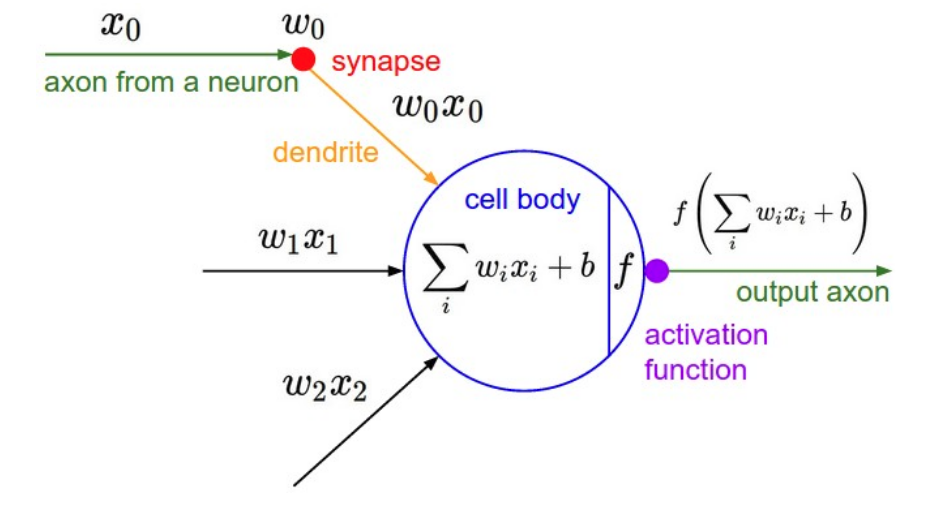
\includegraphics[height=.28\textheight]{Chuong2/Figs/NeuralNetwork.png}
		\label{fig:Neural_Network}
		\caption{Biologically inspired Neural Network \cite{karparthy}}
	\end{center}
\end{figure}

\subsection{Mạng lưới thần kinh nhân tạo}
Lấy ý tưởng từ mạng lưới thần kinh sinh học, cấu trúc của mạng lưới thần kinh nhân tạo (Neural Network: NN) được phát triển để xử lý thông tin tương tự cách bộ não xử lý thông tin. Một khối lượng lớn các quy trình kết nối các phần tử (neural) làm việc cùng nhau làm cho NN có thể giải quyết các vấn đề phức tạp. Giống như con người học từ các ví dụ, NN cũng vậy. Việc học trong hệ thống sinh học là những điều chỉnh các kết nối khớp thần kinh (synaptic) tương tự như việc cập nhật các trọng số trong NN.
Một NN bao gồm 3 lớp: lớp đầu vào (input layer) nơi tiếp nhận dữ liệu, lớp ẩn (hidden layer) để học hỏi cách biểu diễn dữ liệu hợp lý và lớp đầu ra (output) để đưa ra kết quả, dự đoán.Mạng nơ-ron có thể được coi là hệ thống từ đầu đến cuối để tìm ra các đặc trưng trong dữ liệu quá phức tạp để con người có thể nhận ra để dạy cho máy.
\begin{figure}[h]
	\begin{center}
		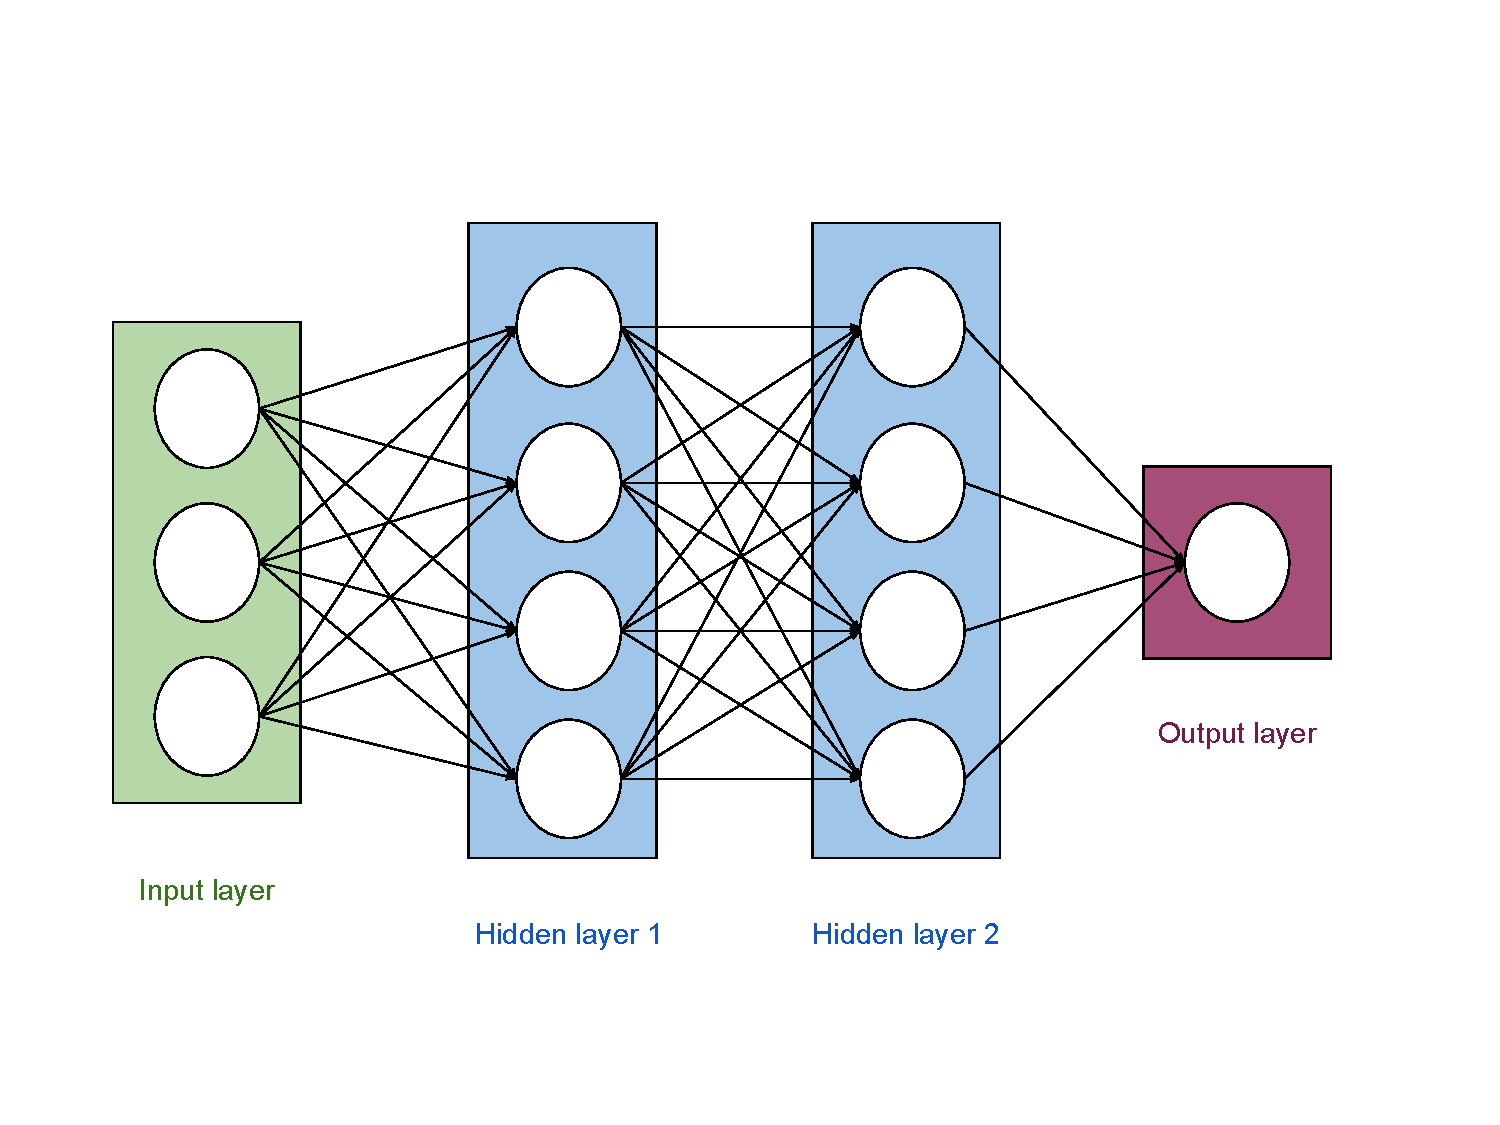
\includegraphics[height=.58\textheight]{Chuong2/Figs/MLP.pdf}
		\label{fig:Two Layered Neural Network}
		\caption{MLP với hai lớp ẩn}
	\end{center}
\end{figure}

\subsubsection{Multi-layer Perceptron (MLP)}
Multi-layer Perceptron (MLP) là dạng đơn giản NN, ta đi qua các khái niệm và ký hiệu:
\begin{enumerate}
	\item Lớp (Layer): Ngoài lớp đầu vào và lớp đầu ra, một MLP có thể có nhiều lớp ẩn (hidden layers) ở giữa. Các lớp ẩn theo thứ tự từ đầu vào đến đầu ra được đánh số thứ tự là Hidden layer 1, Hidden layer 2, ... Hình \eqref{fig:Two Layered Neural Network} là một ví dụ về MLP với 2 lớp ẩn
	\item Units: Một node hình tròn trong một lớp gọi là unit. Unit ở các lớp đầu vào, lớp ẩn và lớp đầu ra. Đầu vào của các lớp ẩn được ký hiệu bỡi $\textit{z}$, đầu ra của mỗi unit thường được ký hiệu bằng $\textit{a}$ (thể hiện hàm activation, tức là giá trị của mỗi unit sau khi ta áp dụng hàm activation). Đầu ra của unit thứ \textit{i} được ký hiệu là $a_{i}^{(l)}$. Giả sử thêm rằng số unit trong lớp thứ $(l)$ là $d^{(l)}$. Vector biểu diễn đầu ra của lớp $l$ được ký hiệu là $\textbf{a}^{(l)}\in \mathbb{R}^{d^{(l)}}$.
	\begin{figure}[h]
		\begin{center}
			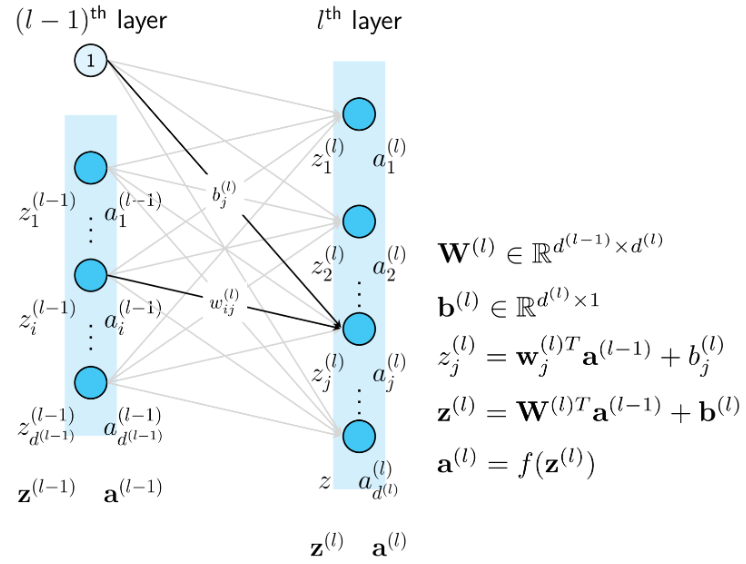
\includegraphics[height=.58\textheight]{Chuong2/Figs/kyhieu.png}
			\label{fig:ky hieu trong MLP}
			\caption{Các ký hiệu sử dụng trong MLP.}
		\end{center}
	\end{figure}
	\item Trọng số và Độ lệch (Weight and Bias): Có $\textbf{L}$ ma trận trọng số cho một MLP có $\textbf{L}$ lớp. Các ma trận này được ký hiệu là $\textbf{W}^{(l)} \in \mathbb{R}^{d^{(l-1)} \times d^{(l)}},l = 1,2,...,L$ trong đó $\textbf{W}^{(l)}$ thể hiện kết nối từ lớp thứ $l=1$ tới lớp thứ $l$ (nếu ta coi lớp đầu vào là lớp 0). Cụ thể hơn, phần tử $w_{ij}^{(l)}$ thể hiện kết nối từ node thứ $i$ của lớp thứ $(l-1)$ tới node thứ $j$ của lớp thứ $(L)$. Các biases của lớp thứ $(l)$ được ký hiệu là $\textbf{b}^{(L)}\in \mathbb{R}^{d^{(l)}}$. Các trọng số này được ký hiệu như trên \ref{fig:ky hieu trong MLP}. Khi tối ưu một MLP cho một công việc nào đó, chúng ta cần tìm các trọng số và biases này. Tập hợp các trọng số và biases lần lượt được ký hiện là $\textbf{W}$ và $\textbf{b}$.
	\item Các hàm kích hoạt (Activation Functions): Mỗi đầu ra của một unit được tính dựa vào công thức:
	\begin{equation}
	a_{i}^{(l)} = f(\textbf{w}_{i}^{(l)T}a^{(l-1)}+b_{i}^{(l)})
	\end{equation}
	Trong đó $f(.)$ là một (không tuyến tính: nonlinear) hàm kích hoạt. Ở dạng vector, biểu thức bên trên được viết là:
	\begin{equation}
	a^{(l)} = f(\textbf{W}^{(l)T}a^{(l-1)}+b^{(l)})
	\end{equation}
	Khi hàm kích hoạt $f(.)$ được áp dụng cho một ma trận (hoặc vector), ta hiểu rằng nó được áp dụng cho từng thành phần của ma trận đó. Sau đó các thành phần này được sắp xếp lại đúng theo thứ tự để được một ma trận có kích thước bằng với ma trận đầu vào.
\end{enumerate}
\subsubsection{Lan truyền ngược(Backpropagation)}
Phương pháp phổ biến nhất để tối ưu MLP vẫn là Gradient Descent(GD). Để áp dụng GD, chúng ta cần tính được gradient của hàm mất mát theo từng ma trận trọng số $\textbf{W}^{(l)}$ và vector bias $\textbf{b}^{(l)}$. Trước hết, chúng ta cần tính dự đoán đầu ra $\hat{y}$ với một đầu vào $x$:

\begin{align*}
\textbf{a}^{(0)} &= x \\
\textit{z}_{i}^{(l)} &= \textbf{w}_{i}^{(l)T}a^{(l-1)}+b_{i}^{(l)} \\
\textbf{z}^{(l)} &= \textbf{W}^{(l)T}a^{(l-1)}+b^{(l)}, l = 1,2,...,L \\
a^{(l)} &= f(\textbf{z}^{(l)}), l = 1,2,...,L\\
\hat{\textbf{y}} &= \textbf{a}^{(L)} \\
\end{align*}

Bước này gọi là feedforward vì cách tính toán được thực hiện từ đầu đến cuối của mạng.
Giả sử $\textit{J}(\textbf{W,b,X,Y})$ là hàm mất mát của bài toán, trong đó $\textbf{W,b}$ là tập hơp tất cả các ma trận trọng số giữa các lớp và biases của mỗi lớp. $\textbf{X,Y}$ là cặp dữ liệu huấn luyện với mỗi cột tương ứng với một điểm dữ liệu. Để có thể áp dụng các phương pháp gradient-based (mà Gradient Descent là một ví dụ). chúng ta cần tính được:
\begin{equation*}
\frac{\partial J}{\partial \textbf{W}^{(l)}}; \frac{\partial J}{\partial \textbf{b}^{(l)}}, l = 1,2,...,L
\end{equation*}
Một ví dụ của hàm mất mát là hàm Mean Square Error (MSE) tức là \textit{trung bình của bình phương lỗi}.
\begin{align*}
\textit{J}(\textbf{W,b,X,Y}) &= \frac{1}{N}\sum_{n=1}^{N} \vert\vert \textbf{y}_{n} - \hat{\textbf{y}}_{n} \vert\vert_{2}^2 \\
&= \frac{1}{N}\sum_{n=1}^{N} \vert\vert \textbf{y}_{n} - \textbf{a}_{n}^{(L)} \vert\vert_{2}^2
\end{align*}
Với $N$ là số cặp dữ liệu $(\textbf{x,y})$ trong tập huấn luyện.

Việc tính toán trực tiếp giá trị này rất phức tạp vè hàm mất mát không phụ thuộc trực tiếp vào các hệ số. Phương pháp phổ biến nhất được dùng có thể là Backpropagation giúp tính gradient từ llopws cuối cùng đến lớp đầu tiên. Lớp cuối cùng được tính toán trước vì nó gần gũi hơn với đầu ra của mô hình và hàm mất mát. Việc tính toán gradient của các lớp trước được thực hiện dựa trên quy tắc đạo hàm của hàm hợp.

Đạo hàm của hàm mất mát theo chỉ một thành phần của ma trận trọng số của lớp cuối cùng:
\begin{align*}
\frac{\partial J}{\partial w_{ij}^{(L)}} &= \frac{\partial J}{\partial z_{j}^{(L)}}.\frac{\partial z_{j}^{(L)}}{\partial w_{ij}^{(L)}} \\
& = e_{j}^{(L)}a_{i}^{(L-1)}
\end{align*}
Trong đó $e_{j}^{(L)} = \frac{\partial J}{\partial z_{j}^{(L)}}$ thường là một đại lượng dễ tính toán và $\frac{\partial z_{j}^{(L)}}{\partial w_{ij}^{(L)}} = a_{i}^{(L-1)}$ vì $z_{j}^{(L)} = \textbf{w}_{j}^{(L)T}\textbf{a}^{(L-1)}+b_{j}^{(L)}$.
Tương tự như thế, đạo hàm của hàm mất mát theo bias của lớp cuối cùng là:
\begin{equation*}
\frac{\partial J}{\partial b_{j}^{(L)}} = \frac{\partial J}{\partial z_{j}^{(L)}}.\frac{\partial z_{j}^{(L)}}{\partial b_{j}^{(L)}} \\
 = e_{j}^{(L)}
\end{equation*}
\begin{figure}[h]
	\begin{center}
		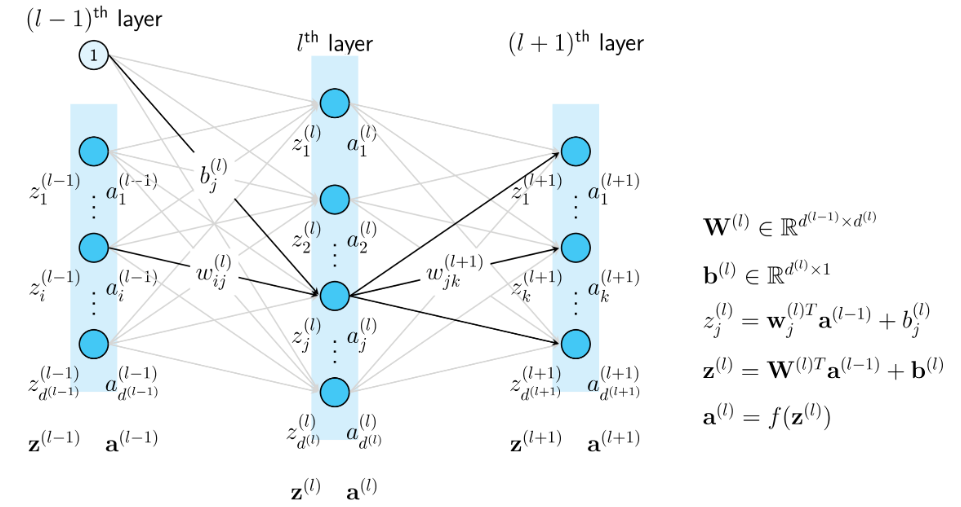
\includegraphics[height=.40\textheight]{Chuong2/Figs/backpropagation.png}
		\label{fig: Mo phong cach tinh backpropagation}
		\caption{Mô phỏng cách tính backpropagation.}
	\end{center}
\end{figure}
Dựa vào hình trên, ta có thể tính được:
\begin{align*}
\frac{\partial J}{\partial w_{ij}^{(l)}} &= \frac{\partial J}{\partial z_{j}^{(l)}}.\frac{\partial z_{j}^{(l)}}{\partial w_{ij}^{(l)}} \\
& = e_{j}^{(l)}a_{i}^{(l-1)}
\end{align*}
với:
\begin{align*}
e_{j}^{(l)} &= \frac{\partial J}{\partial z_{j}^{(l)}}= \frac{\partial J}{\partial a_{j}^{(l)}}.\frac{\partial a_{j}^{(l)}}{\partial z_{j}^{(l)}}\\
& = (\sum_{k=1}^{d^{(l+1)}}\frac{\partial J}{\partial z_{k}^{(l+1)}}.\frac{\partial z_{k}^{(l+1)}}{\partial a_{j}^{(l)}})f^{'}(z_{j}^{(l)})\\
& = (\sum_{k=1}^{d^{(l+1)}}e_{k}^{(l+1)}w_{jk}^{(l+1)})f^{'}(z_{j}^{(l)})\\
& = (\textbf{w}_j^{(l+1)}\textbf{e}^{(l+1)})f^{'}(z_{j}^{(l)})
\end{align*}
trong đó $\textbf{e}^{(l+1)}=[e_{1}^{(l+1)},e_{2}^{(l+1)},...,e_{d^{(l+1)}}^{(l+1)}]^T \in \mathbb{R}^{d^{(l+1)}\time 1}$ và $\textbf{w}_{j:}^{(l+1)}$ được hiểu là hàng thứ \textit{j} của ma trận $\textbf{W}^{(l+1)}$
Với cách làm tương tự, ta có thể suy ra:
\begin{equation*}
\frac{\partial J}{\partial b_{j}^{(l)}} = e_j^{(l)}
\end{equation*}
Nhận thấy rằng trong các công thức trên đây, việc tính $e_j^{(l)}$ đóng một vai trò quan trọng, Hơn nữa, để tính được các giá trị này, ta cần tính được các $e_j^{(l+1)}$. Nói cách khác, ta cần tính ngược các giá trị này từ cuối.
\subsubsection{Convolutional Neural Network}

Vấn đề chính của lớp FC là cần quá nhiều trọng số, làm khối lượng của mô hình lớn đối mặt với những vẫn đề như thời gian đào tạo (training) và đưa ra dự đoán của mô hình chậm và đặc biệt dễ bị overfitting,...
Ví dụ: trọng nhiệm vụ phân loại ảnh, đầu vào là một ảnh có kích thước $64\times64\times3$, FC cần 12288 trọng số cho một đầu ra trong lớp ẩn đầu tiên. Số lượng trọng số sẽ tăng lên rất nhiều lần khi kích thước ảnh tăng.
Ngoài ra, lớp FC còn làm mất thông tin hình học của bức ảnh vì đang xem các điểm ảnh (pixel) độc lập với nhau. Nhưng trong thực tế, các pixel trong từng vùng nhỏ (local) có ảnh hưởng đến nhau. 
Convolutional Neural Network(CNN) được thiết kế ra để giải quyết các vấn đề của FC trong phân loại ảnh.
CNN thường bao gồm các thành phần sau:
\begin{enumerate}
	\item Lớp đầu vào: một ảnh RGB có kích thước $H \times W \times 3$  tương ứng $Height \times Width \times Chanels$.
	\item Khối convolution: bao gồm
	\begin{enumerate}
		\item Lớp convolution: sử dụng một ma trận lọc (kernel hoặc fillters) có kích thước nhỏ, thường là $3\times 3$ hoặc $5\times5$, trượt qua lần lượt khắp ảnh hoặc bản đồ đặc trưng (feature map), thực hiện phép nhân tích chập cho kernel và một phần nhỏ cùng kích thước với kernel trên ảnh, tổng của ma trận tích vừa thu được được xem như một phần tử đầu ra tương ứng trên lớp đó.
		\begin{figure}[h]
			\begin{center}
				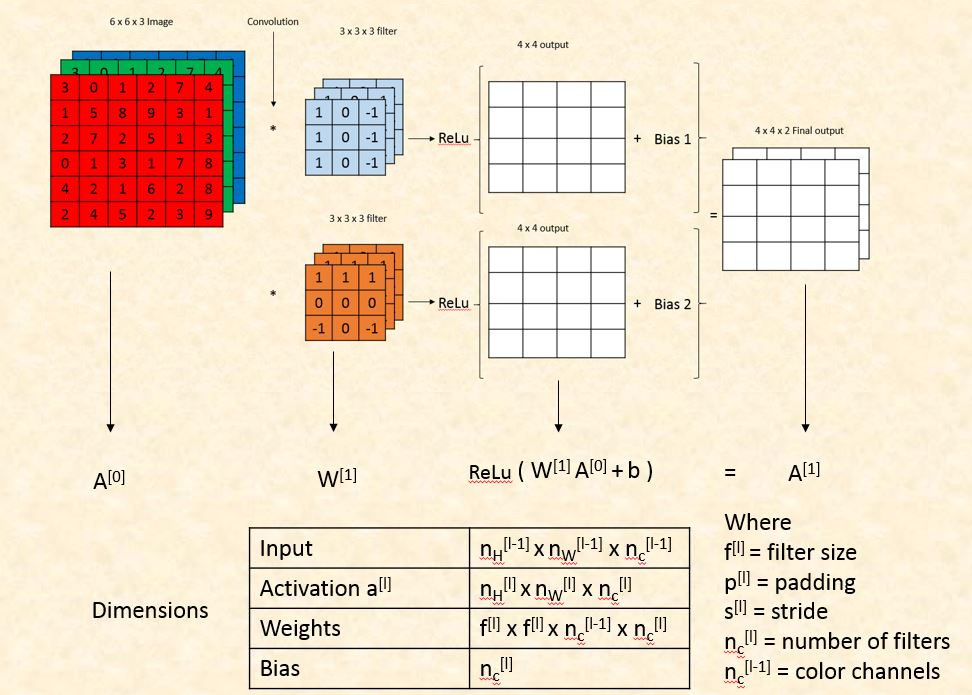
\includegraphics[height=.28\textheight]{Chuong2/Figs/Convolution-Layer-Dimensions.jpg}
				\label{fig:convolution layer}
				\caption{Kích thước tham số của lớp convolution \cite{karparthy}}
			\end{center}
		\end{figure}
		\item Hàm kích hoạt (activation function): thường sử dụng hàm ReLU, được mô tả như hàm $max(0,x)$. Có nghĩa là bất kỳ số thực nào bé hơn 0 được chuyển về 0 trong khi những số thực lớn hơn 0 được giữ nguyên giá trị.
		\item Lớp tổng hợp (Pooling layer): lớp pooling được sử dụng để đơn giản hóa thông tin đầu ra, giảm bớt số lượng neuron. Max-pooling được sử dụng phổ biến nhất, nó chọn giá trị lớn nhất trong vùng đầu vào $2\times 2$. Như vậy, qua lớp max-pooling thì số lượng neuron giảm đi phân nửa. Chúng ta có thể thấy rằng max-pooling lọc những đặc trưng yếu, chỉ giữ lại đặc trưng mạnh nhất.
		\begin{figure}[h]
			\begin{center}
				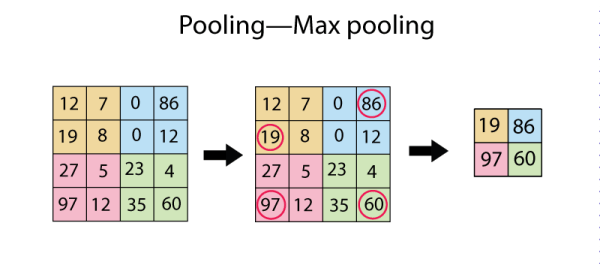
\includegraphics[height=.28\textheight]{Chuong2/Figs/poolingmax.png}
				\label{fig:maxpooling layer}
				\caption{Một ví dụ của lớp max-pooling}
			\end{center}
		\end{figure}
		
	\end{enumerate}
	\item Lớp FC
\end{enumerate}
Trong một mạng CNN, thông thường các lớp được sắp xếp theo thứ tự: lớp đầu vào + một vài khối convolution + lớp FC + lớp đầu ra.
\begin{figure}[h]
	\begin{center}
		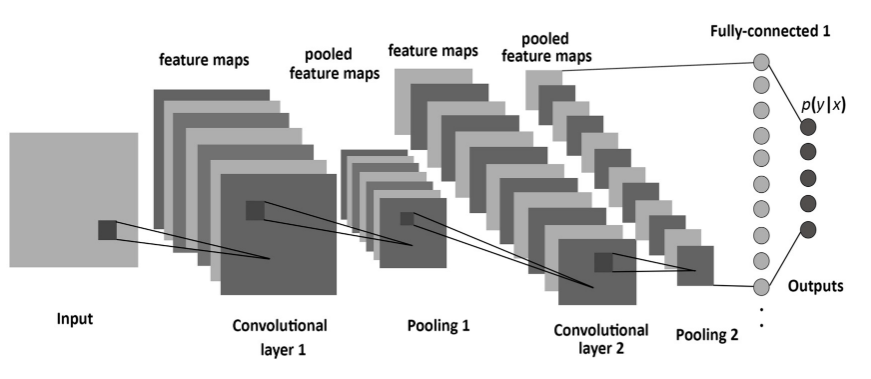
\includegraphics[height=.28\textheight]{Chuong2/Figs/CNN.png}
		\label{fig:CNN}
		\caption{Cấu trúc đầy đủ của một mạng CNN}
	\end{center}
\end{figure}



\section{Khoảng cách giữa hai phân phối}
\subsection{Entropy và cross-entropy}
Entropy là một khái niệm thường gặp trong lý thuyết thông tin. Chúng dùng để đo lượng thông tin mang lại của một sự kiện hay đặc trưng khi biết phân phối xác suất của chúng.
Với một phân phối P,
\begin{equation*}
Entropy = H(P) = \mathbb{E}_{x\sim P}[-logP(x)]
\end{equation*}
Miến là ta biết phân phối xác suất của bất kỳ cái gì, ta đều có thể tính toán entropy của nó.

Trong trường hợp phân phối xác suât thật P ta không biết hoặc rất khó để tính toán, việc tìm được một phân phối Q xấp xỉ P rất có ý nghĩa. Từ đó, ta cần phải định nghĩa một độ đo giữa hai phân phối để có thể đánh giá được việc xấp sỉ P băng Q có hiệu quả hạy chưa?
Ta định nghĩa:
\begin{equation*}
CrossEntropy = H(P,Q) = \mathbb{E}_{x\sim P}[-logQ(x)]
\end{equation*}
CrossEntropy là lượng thông tin mang lại của của sự kiện có phân phối xấp xỉ Q nhưng được lấy mẫu với phân phối thực P.
Lúc này, việc so sánh giữa CrossEntropy và Entropy có ý nghĩa vì chúng đều được lẫy mẫu từ cùng một phân phối.
\subsection{Phân kỳ Kullback-Leibler}
Phân kỳ Kullback-Leibler cho chúng ta biết phân phối Q xấp xỉ phân phối P tốt như thế nào bằng cách tính toán cross-entropy trừ entropy.
\begin{align*}
D_KL(P||Q) &= H(P,Q) - H(P)\\
& = \mathbb{E}_{x\sim P}[-logQ(x)] - \mathbb{E}_{x\sim P}[-logP(x)]\\
& = \mathbb{E}_{x\sim P}[logP(x)-logQ(x)]\\
& = \mathbb{E}_{x\sim P}[log\frac{P(x)}{Q(x)}]
\end{align*}
Phân kỳ KL đo lượng thông tin chênh lệch hay sự không hiệu quá khi sử dụng phân phối Q để xấp xỉ phân phối P.
\begin{figure}[h]
	\begin{center}
		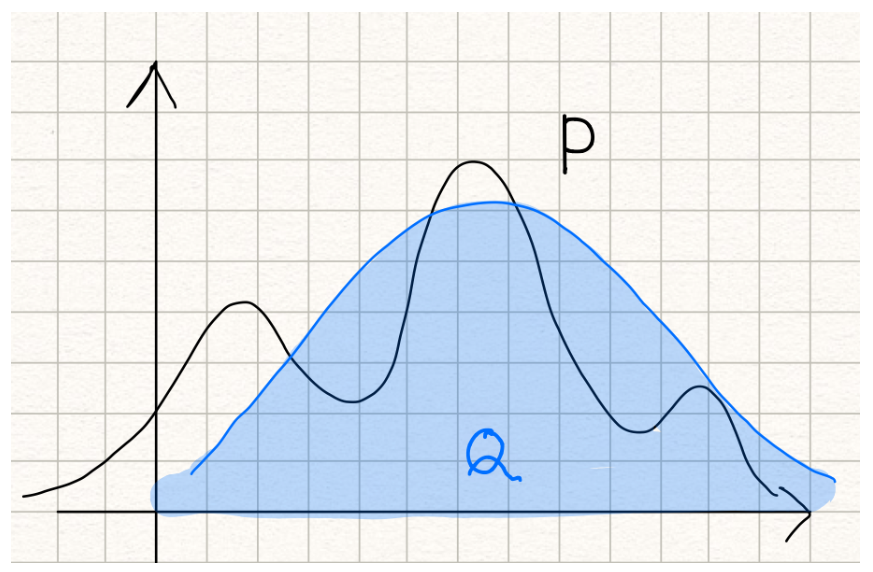
\includegraphics[height=.28\textheight]{Chuong2/Figs/KL.png}
		\label{fig:KL}
		\caption{Xấp xỉ phân phối P bằng Q}
	\end{center}
\end{figure}



% !TeX spellcheck = en_US

%!TEX root = ../thesis.tex
%*******************************************************************************
%****************************** Second Chapter *********************************
%*******************************************************************************


\chapter{Statistical inference}

\pagebreak

\section{Bayesian Inference}
\subsection{Định lý Bayes}
Định lý Bayes là một định lý cơ bản thường xuyên được sử dụng trong lý thuyết học máy.

\begin{equation}
	P(A/B) = \frac{P(B/A)P(A)}{P(B)}
\end{equation}
Trong đó: 
A và B là các sự kiện.

$P(A), P(B)$ : Xác suất của sự kiện A, B xảy ra tương ứng.

$P(A/B)$ là xác suất sự kiện A xảy ra nếu biết sự kiện B đã xảy ra

$P(B/A)$ là xác suất sự kiện B xảy ra nếu biết sự kiện A đã xảy ra

Định lý Bayes cho phép chúng ta sử dụng những kiến thức hay niềm tin đã có để tính toán xác suất cho một sự kiện nào đó.
\subsection{Suy luận Bayesian}
Suy luận Bayes là một phương pháp suy luận thống kê mà định lý Bayes được sử dụng để cập nhật xác suất của một giả thuyết khi có thêm nhiều thông tin hay bằng chứng hơn. 

Một phần quan trọng của suy luận Bayes là việc thiết lập các tham số và mô hình. Mô hình là một công thức toán học của bộ dữ liệu quan sát được. Tham số là các yếu tố trong mô hình ảnh hưởng đến dữ liệu.
Để xây dựng một mô hình, ta cần thiết kế cấu trúc và ước lượng bộ tham số của nó.
Giá sử $\Theta$ đại diện cho bộ tham số của mô hình, $y = \{y_1, y_2, \dots, y_n \}$ là bộ dữ liệu mà chúng ta có được. Lúc này, định lý Bayes được viết dưới dạng:
\begin{equation}
P(\Theta/y) = \frac{P(y/\Theta)P(\Theta)}{P(y)}
\end{equation}
$P(y/\Theta)$ được gọi là \textit{Likelihood}, mô tả tính hợp lý của giá trị tham số mô hình từ các dữ liệu quan sát được.

$P(\Theta)$ được gọi là phân phối tiền nghiệm hay \textit{prior}, đại diện cho những kiến thức, niềm tin về giá trị thực của tham số từ những kinh nghiệm trước đây khi chưa tiếp xúc với dữ liệu hiện tại.

$P(\Theta/y)$ được gọi là phân phối hậu nghiệm hay \textit{posterior}. Nó đại diện cho phân phối của các tham số sau khi đã quan sát được bộ dữ liệu \textit{y}.

$P(y)$ được gọi là phân phối cận biên hay chứng cứ, nó giúp chuẩn hóa đầu ra của \textit{posterior}, đảm bảo \textit{posterior} thõa điều kiện là một phân phối xác suất.

Trong một vài trường hợp, chúng ta không quan tâm đến việc liệu phân phối có được chuẩn hóa hay không. Khí đó, chúng ta có thể viết lại định lý Bayes dưới dạng rút gọn hơn:
\begin{equation}
P(\Theta/y) \propto P(y/\Theta)P(\Theta)
\end{equation}
\textit{Một số lưu lý về prior}
\textit{Prior} là một sự đặc biệt trong suy luận Bayes, giúp đưa những kiến thức đã biết hay kiến thức của chuyên gia về $\Theta$ vào việc hình thành nên mô hình, làm cho mô hình thu được không phụ thuộc hoàn toàn dữ liệu, ngăn chặn được tình trạng \textit{overfitting} khi có ít dữ liệu.

\textit{Prior} có nhiệm vụ bảo vệ (một phần nào đó) kiến thức đã có về mô hình khỏi những dữ liệu nhiễu. \textit{Prior} có sức ảnh hưởng mạnh nhất khi mô hình chưa được học với quá nhiều dữ liệu.
\begin{figure}[h]
	\begin{center}
		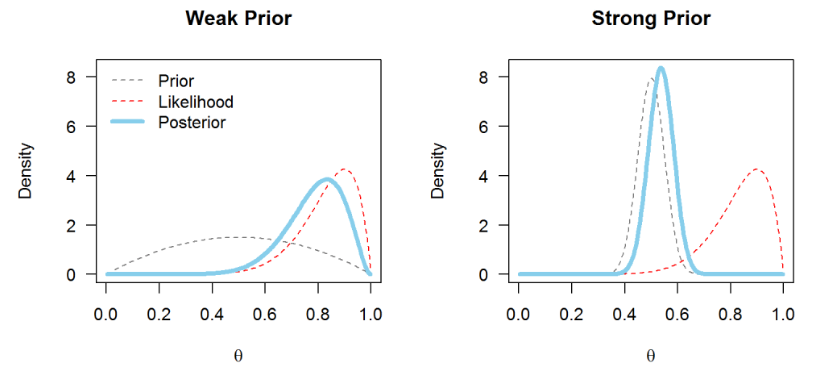
\includegraphics[height=.25\textheight]{Chuong3/Figs/prior.png}
		\label{fig:su anh huong cua prior}
		\caption{Sự ảnh hưởng của một \textit{prior} yếu và một \textit{prior} mạnh khi tung đồng xu được 9/10 mặt ngửa}
	\end{center}
\end{figure}
Trong thực thế, đặc biệt là trong việc đào tạo mô hình, việc nhận định sai về $\Theta$ hay Prior sai rất dễ xảy ra. Trong trường hợp này, chỉ cần thu thập thật nhiều dữ liệu. Khi ấy, sự ảnh hưởng của Prior ngày càng giảm dần, Posterior vẫn sẽ hội tụ đến đến điểm tối ưu. Điều này được minh họa ở hình \ref{fig:su anh huong cua prior sai}
\begin{figure}[h]
	\begin{subfigure}{.5\textwidth}
	\centering
	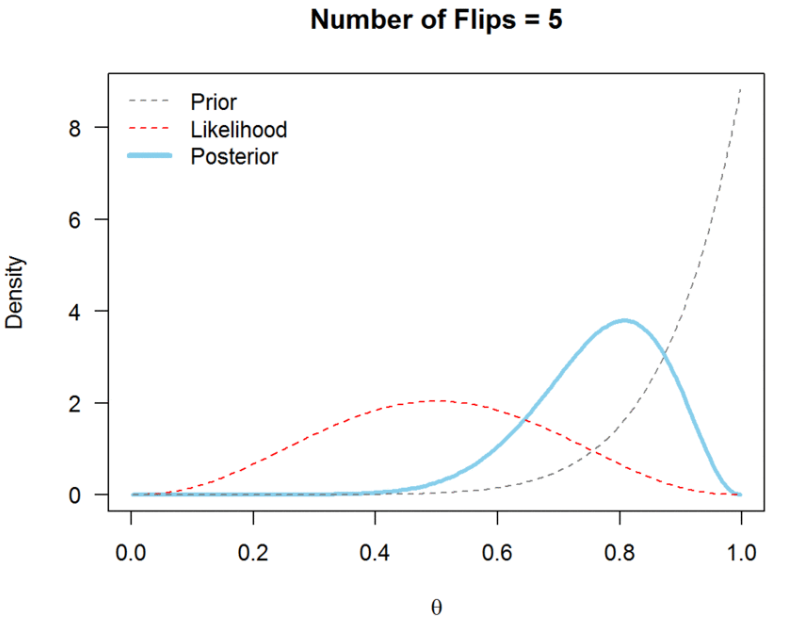
\includegraphics[width=.8\linewidth]{Chuong3/Figs/5.png}
	\label{fig:sfig1}
	\end{subfigure}
	\begin{subfigure}{.5\textwidth}
	\centering
	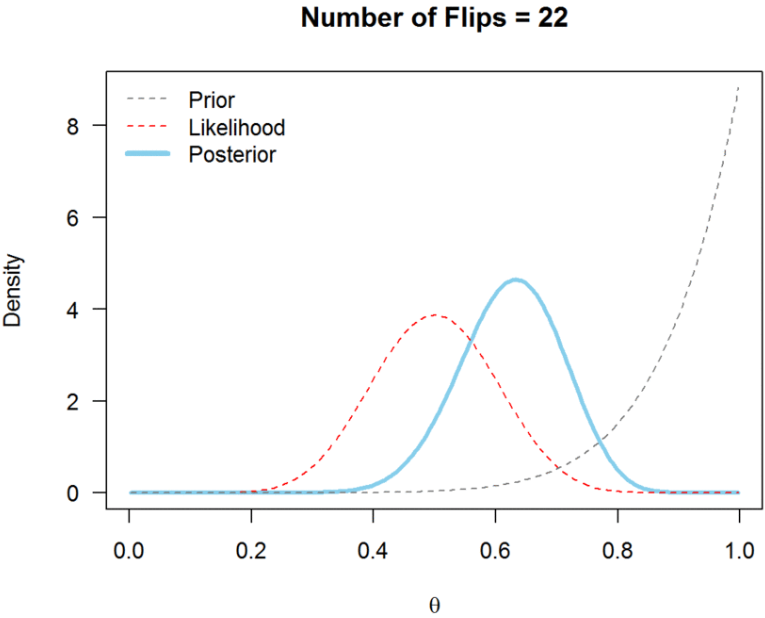
\includegraphics[width=.8\linewidth]{Chuong3/Figs/22.png}
	\label{fig:sfig1}
	\end{subfigure}
	\begin{subfigure}{.5\textwidth}
	\centering
	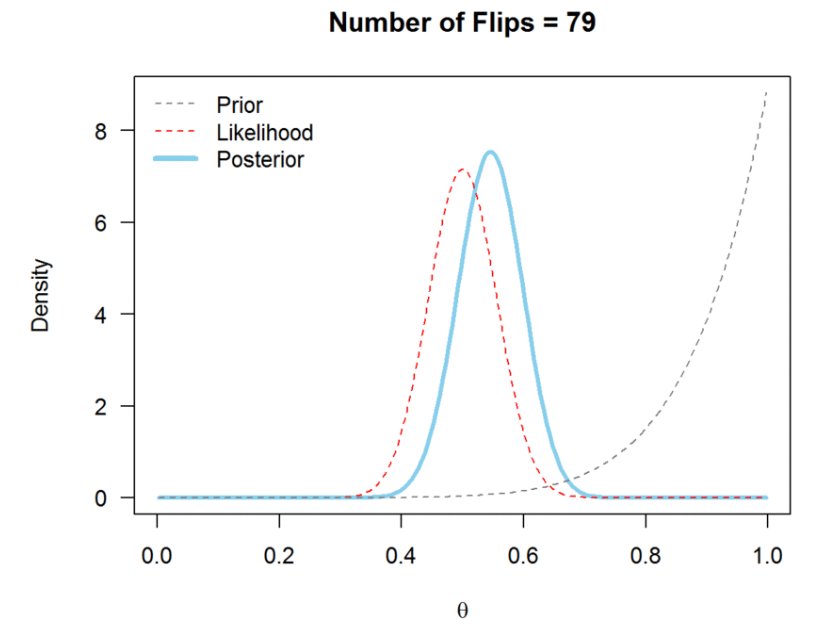
\includegraphics[width=.8\linewidth]{Chuong3/Figs/79.png}
	\label{fig:sfig1}
	\end{subfigure}
	\begin{subfigure}{.5\textwidth}
	\centering
	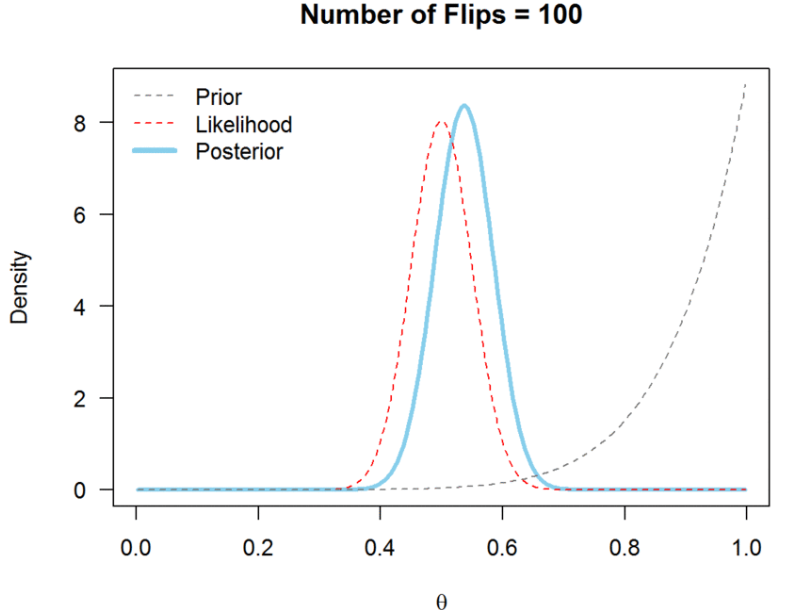
\includegraphics[width=.8\linewidth]{Chuong3/Figs/100.png}
	\label{fig:sfig1}
	\end{subfigure}
	\label{fig:su anh huong cua prior sai}
	\caption{Cùng với một prior khá lệch, khi ta tung đồng xu càng nhiều thì posterior càng hội tụ đến LikeLihood}
\end{figure}


\section{Variational Inference}
\subsection{Probabilistic model}
Một mạng thần kinh có thể được xem như mộng mô hình xác suất $p(y/x,w)$. Trong nhiệm vụ phân loại, $y$ là tập hợp các phân lớp và  $p(y/x,w)$ là một phân phối phân loại. Trong nhiệm vụ hồi quy, $y$ là một biến liên tục và  $p(y/x,w)$ là một phân phối Gaussian.

Cho tập dữ liệu đào tạo $\mathcal{D}={\textbf{x}^{(i)},y^{(i)}}$, chúng ta có thể xây dựng Likelihood $p(\mathcal{D}/\textbf{w}) = \prod_{i}p(y^{(i)}|\textbf{x}^{(i)},\textbf{w})$ là một hàm số của $\textbf{w}$. Cực đại hóa Likelihood (MLE) cũng là một phương pháp hay dùng để tìm $\textbf{w}$ tối ưu nhưng nó dễ dẫn đến onverfiting vì phụ thuộc hoàn toàn vào dữ liệu.

Nhân Likelihood với một Prior $p(\textbf{w})$ sẽ tỷ lệ với phân phối Posterior $p(\textbf{w}/\mathcal{D}) \propto p(\mathcal(D/\textbf{w})p(\textbf{w}))$. Cực đại hóa $p(\mathcal(D/\textbf{w})p(\textbf{w}))$ tương đương bởi tìm $\textbf{w}$ để Posterior $p(\textbf{w}/\mathcal{D})$ đạt giá trị lớn nhất (hay được gọi là MAP). Làm việc với MAP cho hiệu quả tổng quát hơn và có thể ngăn chặn overfitting.

MLE và MAP đều ước lượng điểm cho các tham số trong mô hình. Thay vào đó, nếu chúng ta có phân phối Posterior đầy đủ cho tất cả các tham số, chúng ta có thể đưa ra nhiều dự đoán với những tham số được lấy ngẫu nhiên từ Posterior. Khi ấy, không những ta thu được dự đoán có tính tổng quát cao mà còn đánh giá được độ không chắc chắn của dự đoán ấy. Khi đó, mục tiêu tối ưu hóa hay hàm mất mát được viết dưới dạng
\begin{equation*}
p(y/\textbf{x},\mathcal{D}) = \int p(y/\textbf{x},\textbf{w})p(\textbf{w}/\mathcal{D})d\textbf{w}
\end{equation*}
Điều này tương đương với trung bình các dự đoán đến từ các mạng thần kinh có trong số được lấy từ phân phối Posterior.
\subsection{Variational Inference}
Thật không may, việc ước lượng Posterior $p(y/\textbf{x},\mathcal{D})$ trong mạng thần kinh rất khó khăn vì trong đó, số lượng tham số rất lớn, có thể đến hàng triệu tham số. Vì thế, chúng ta phải ước lượng Posterior bằng một phân phối $p(\textbf{w}/\theta)$ có dạng đơn giản hơn. Việc cực tiểu hóa KL divergence giữa $p(\textbf{w}/\theta)$ và phân phối Posterior $p(y/\textbf{x},\mathcal{D})$ có thể giúp ta làm việc này. Nhiệm vụ của ta là tìm điểm tối ưu $\theta^*$ của $\theta$ để KL divergence đạt cực tiểu.
\begin{align*}
\theta^* &= \arg\min_{\theta}\textbf{KL}[q(\textbf{w}|\theta)||P(\textbf{w}|\mathcal{D})] \\
& = \arg\min_{\theta}\displaystyle \int q(\textbf{w}|\theta)log\frac{q(\textbf{w}|\theta)P(\mathcal{D})}{P(\textbf{w})P(\mathcal{D}|\textbf{w})}d\textbf{w} \\
& = \arg\min_{\theta}\displaystyle \int q(\textbf{w}|\theta)(log\frac{q(\textbf{w}|\theta)}{P(\textbf{w})}-log(P(\mathcal{D}|\textbf{w}))+ log(P(\mathcal{D})))d\textbf{w} \\
& = \arg\min_{\theta}\textbf{KL}[q(\textbf{w}|\theta)||P(\textbf{w})] - \mathbb{E}_{q(\textbf{w}|\theta)}[\log P(\mathcal{D}|\textbf{w})] + \mathbb{E}_{q(\textbf{w}|\theta)}[\log P(\mathcal{D})] \\
& = \arg\min_{\theta}\textbf{KL}[q(\textbf{w}|\theta)||P(\textbf{w})] - \mathbb{E}_{q(\textbf{w}|\theta)}[\log P(\mathcal{D}|\textbf{w})] \\
\end{align*}
$\log P(\mathcal{D})$ có thể được bỏ qua trong việc tối ưu hóa vì nó là hằng số.
Để đơn giản, ta có thể định nghĩa hàm mất mát:
\begin{align*}
\mathcal{F}(\mathcal{D},\theta) &= \textbf{KL}[q(\textbf{w}|\theta)||p(\textbf{w})] - \mathbb{E}_{q(\textbf{w}|\theta)}[\log P(\mathcal{D}|\textbf{w})]  \\
& = \mathbb{E}_{q(\textbf{w}|\theta)}\log p(w|\theta) - \mathbb{E}_{q(\textbf{w}|\theta)}\log p(w) - \mathbb{E}_{q(\textbf{w}|\theta)}\log p(\mathcal{D}|\textbf{w}) \\
& \approx\frac{1}{N}\sum_{i = 1}^{N}[\log p(w^{(i)}|\theta) - \log p(w^{(i)}) - \log p(\mathcal{D}|w^{(i)})]\\
\end{align*}
\section{Uncertainties in Bayesian Learning}

Sự không chắc chắn của một mạng thần kinh là độ đo thể hiện sự chắc chắn bao nhiêu của mô hình với dự đoán của nó. Trong mô hình Bayesian, có 2 loại không chắc chắn chính: Aleatoric và Epistemic.

Độ không chắc chắn Aleatoric nắm bắt sự không chắc chắn đối với thông tin mà dữ liệu không thể giải thích. Ví dụ, trong các vấn đề với ảnh, các vị trí mà đối tượng bị che khuất hoặc thiếu các đặc điểm nhận dạng thường có đô không chắn chắn Aleatoric cao. Aleatoric rất quan trọng trong các trường hợp:
\begin{enumerate}
	\item Dữ liệu lớn, khi ấy Epistemic hầu như rất thấp cho mọi dữ liệu.
	\item Các ứng dụng real-time, vì Aleatoric có thể được mô hình hóa như một hàm xác định của đầu vào, không cần phải lấy mẫu nhiều lần.
\end{enumerate}


Độ không chắc chắn Epistemic nắm bắt sự thiếu hiểu biết của chúng tôi về mô hình nào tạo ra dữ liệu thu thập được. Sự không chắc chắn này có thể được giải thích bởi việc cung cấp thêm dữ liệu và thường được gọi là sự không chắc chắn của mô hình. Epistemic thường quan trọng để mô hình hóa cho:

\begin{enumerate}
	\item Các ứng dụng yêu cầu sự an toàn, Vì Epistemic có thể
	\item Dữ liệu nhỏ và thưa thớt.
\end{enumerate}

\begin{figure}[h]
	\begin{center}
		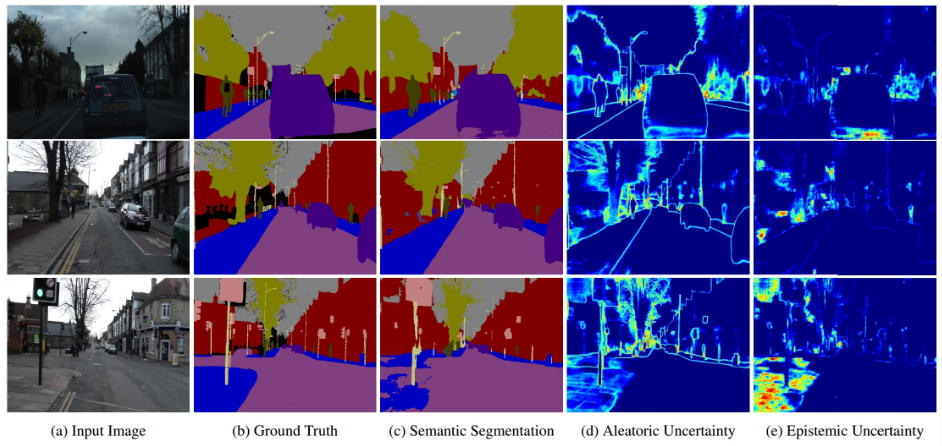
\includegraphics[height=.25\textheight]{Chuong3/Figs/uncertainty.png}
		\label{fig:minh hoa uncertainty}
		\caption{Một ví dụ của uncertainty trong bài toán Semamtation}
	\end{center}
\end{figure}



% !TeX spellcheck = en_US

%!TEX root = ../thesis.tex
%*******************************************************************************
%****************************** Second Chapter *********************************
%*******************************************************************************


\chapter{Bayesian Neural Network}

\pagebreak

\section{Bayesian Inference}
\subsection{Định lý Bayes}
Định lý Bayes là một định lý cơ bản thường xuyên được sử dụng trong lý thuyết học máy.

\begin{equation}
	P(A/B) = \frac{P(B/A)P(A)}{P(B)}
\end{equation}
Trong đó: 
A và B là các sự kiện.

$P(A), P(B)$ : Xác suất của sự kiện A, B xảy ra tương ứng.

$P(A/B)$ là xác suất sự kiện A xảy ra nếu biết sự kiện B đã xảy ra

$P(B/A)$ là xác suất sự kiện B xảy ra nếu biết sự kiện A đã xảy ra

Định lý Bayes cho phép chúng ta sử dụng những kiến thức hay niềm tin đã có để tính toán xác suất cho một sự kiện nào đó.
\subsection{Suy luận Bayesian}
Suy luận Bayes là một phương pháp suy luận thống kê mà định lý Bayes được sử dụng để cập nhật xác suất của một giả thuyết khi có thêm nhiều thông tin hay bằng chứng hơn. 

Một phần quan trọng của suy luận Bayes là việc thiết lập các tham số và mô hình. Mô hình là một công thức toán học của bộ dữ liệu quan sát được. Tham số là các yếu tố trong mô hình ảnh hưởng đến dữ liệu.
Để xây dựng một mô hình, ta cần thiết kế cấu trúc và ước lượng bộ tham số của nó.
Giá sử $\Theta$ đại diện cho bộ tham số của mô hình, $y = \{y_1, y_2, \dots, y_n \}$ là bộ dữ liệu mà chúng ta có được. Lúc này, định lý Bayes được viết dưới dạng:
\begin{equation}
P(\Theta/y) = \frac{P(y/\Theta)P(\Theta)}{P(y)}
\end{equation}
$P(y/\Theta)$ được gọi là \textit{Likelihood}, mô tả tính hợp lý của giá trị tham số mô hình từ các dữ liệu quan sát được.

$P(\Theta)$ được gọi là phân phối tiền nghiệm hay \textit{prior}, đại diện cho những kiến thức, niềm tin về giá trị thực của tham số từ những kinh nghiệm trước đây khi chưa tiếp xúc với dữ liệu hiện tại.

$P(\Theta/y)$ được gọi là phân phối hậu nghiệm hay \textit{posterior}. Nó đại diện cho phân phối của các tham số sau khi đã quan sát được bộ dữ liệu \textit{y}.

$P(y)$ được gọi là phân phối cận biên hay chứng cứ, nó giúp chuẩn hóa đầu ra của \textit{posterior}, đảm bảo \textit{posterior} thõa điều kiện là một phân phối xác suất.

Trong một vài trường hợp, chúng ta không quan tâm đến việc liệu phân phối có được chuẩn hóa hay không. Khí đó, chúng ta có thể viết lại định lý Bayes dưới dạng rút gọn hơn:
\begin{equation}
P(\Theta/y) \propto P(y/\Theta)P(\Theta)
\end{equation}
\textit{Một số lưu lý về prior}
\textit{Prior} là một sự đặc biệt trong suy luận Bayes, giúp đưa những kiến thức đã biết hay kiến thức của chuyên gia về $\Theta$ vào việc hình thành nên mô hình, làm cho mô hình thu được không phụ thuộc hoàn toàn dữ liệu, ngăn chặn được tình trạng \textit{overfitting} khi có ít dữ liệu.

\textit{Prior} có nhiệm vụ bảo vệ (một phần nào đó) kiến thức đã có về mô hình khỏi những dữ liệu nhiễu. \textit{Prior} có sức ảnh hưởng mạnh nhất khi mô hình chưa được học với quá nhiều dữ liệu.
\begin{figure}[h]
	\begin{center}
		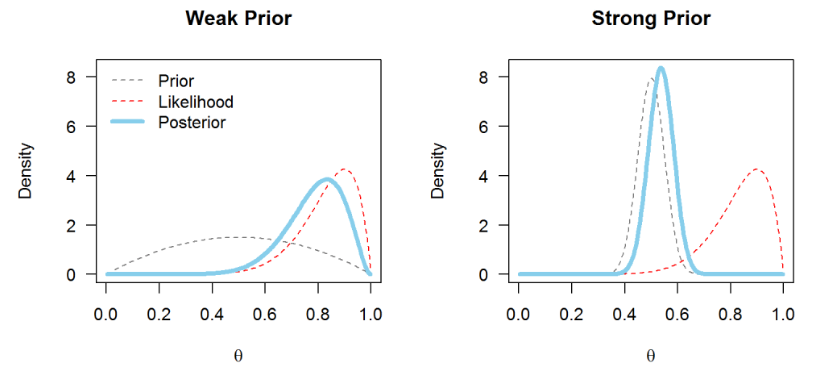
\includegraphics[height=.25\textheight]{Chuong3/Figs/prior.png}
		\label{fig:su anh huong cua prior}
		\caption{Sự ảnh hưởng của một \textit{prior} yếu và một \textit{prior} mạnh khi tung đồng xu được 9/10 mặt ngửa}
	\end{center}
\end{figure}
Trong thực thế, đặc biệt là trong việc đào tạo mô hình, việc nhận định sai về $\Theta$ hay Prior sai rất dễ xảy ra. Trong trường hợp này, chỉ cần thu thập thật nhiều dữ liệu. Khi ấy, sự ảnh hưởng của Prior ngày càng giảm dần, Posterior vẫn sẽ hội tụ đến đến điểm tối ưu. Điều này được minh họa ở hình \ref{fig:su anh huong cua prior sai}
\begin{figure}[h]
	\begin{subfigure}{.5\textwidth}
	\centering
	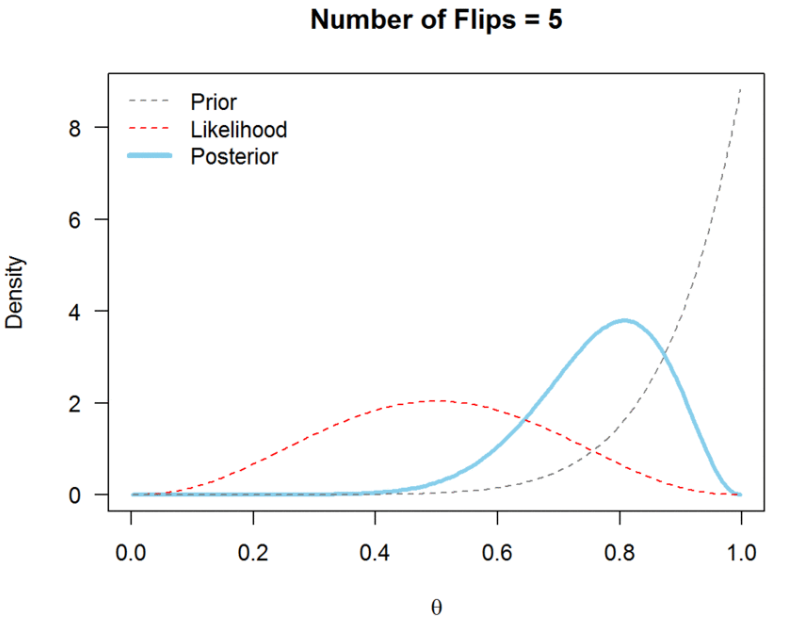
\includegraphics[width=.8\linewidth]{Chuong3/Figs/5.png}
	\label{fig:sfig1}
	\end{subfigure}
	\begin{subfigure}{.5\textwidth}
	\centering
	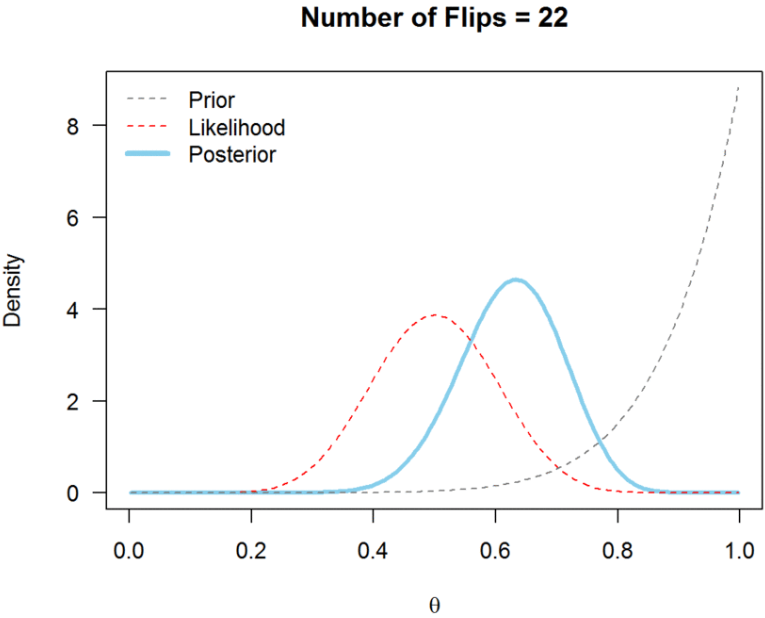
\includegraphics[width=.8\linewidth]{Chuong3/Figs/22.png}
	\label{fig:sfig1}
	\end{subfigure}
	\begin{subfigure}{.5\textwidth}
	\centering
	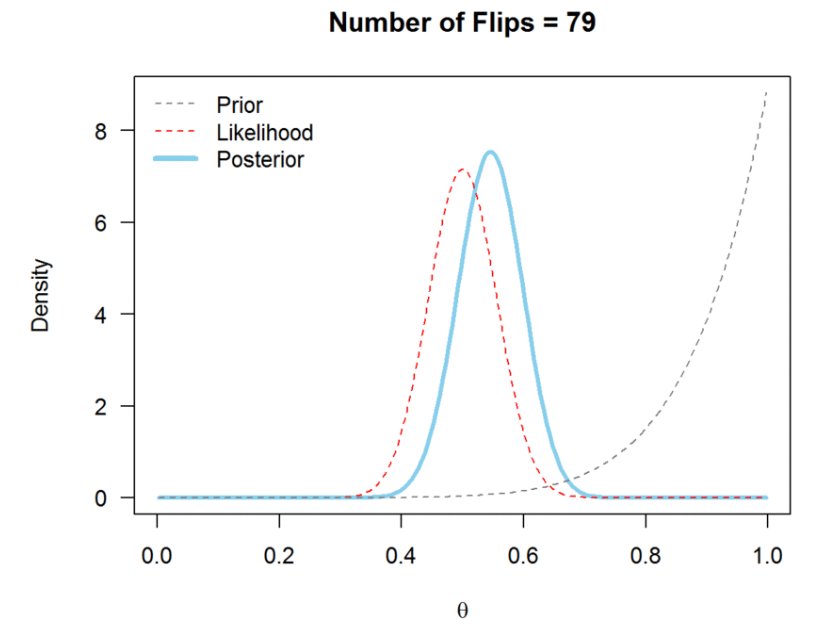
\includegraphics[width=.8\linewidth]{Chuong3/Figs/79.png}
	\label{fig:sfig1}
	\end{subfigure}
	\begin{subfigure}{.5\textwidth}
	\centering
	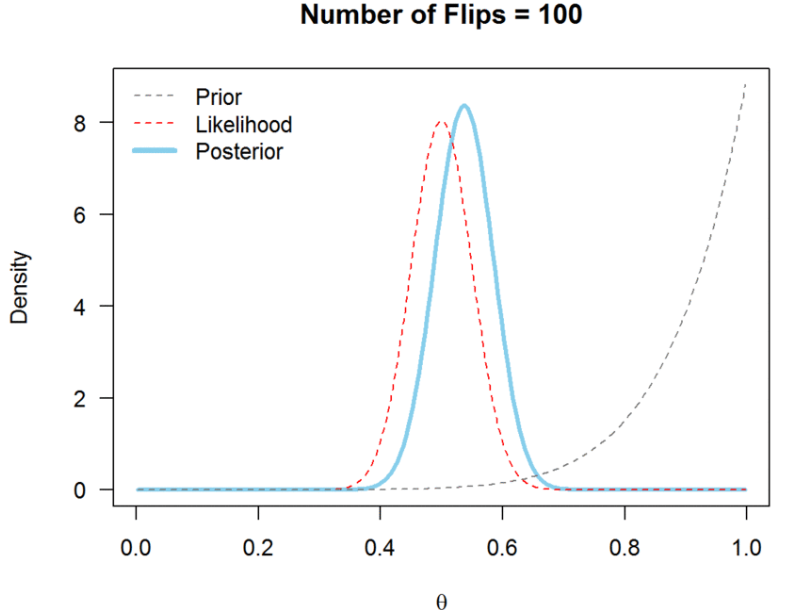
\includegraphics[width=.8\linewidth]{Chuong3/Figs/100.png}
	\label{fig:sfig1}
	\end{subfigure}
	\label{fig:su anh huong cua prior sai}
	\caption{Cùng với một prior khá lệch, khi ta tung đồng xu càng nhiều thì posterior càng hội tụ đến LikeLihood}
\end{figure}


\section{Variational Inference}
\subsection{Probabilistic model}
Một mạng thần kinh có thể được xem như mộng mô hình xác suất $p(y/x,w)$. Trong nhiệm vụ phân loại, $y$ là tập hợp các phân lớp và  $p(y/x,w)$ là một phân phối phân loại. Trong nhiệm vụ hồi quy, $y$ là một biến liên tục và  $p(y/x,w)$ là một phân phối Gaussian.

Cho tập dữ liệu đào tạo $\mathcal{D}={\textbf{x}^{(i)},y^{(i)}}$, chúng ta có thể xây dựng Likelihood $p(\mathcal{D}/\textbf{w}) = \prod_{i}p(y^{(i)}|\textbf{x}^{(i)},\textbf{w})$ là một hàm số của $\textbf{w}$. Cực đại hóa Likelihood (MLE) cũng là một phương pháp hay dùng để tìm $\textbf{w}$ tối ưu nhưng nó dễ dẫn đến onverfiting vì phụ thuộc hoàn toàn vào dữ liệu.

Nhân Likelihood với một Prior $p(\textbf{w})$ sẽ tỷ lệ với phân phối Posterior $p(\textbf{w}/\mathcal{D}) \propto p(\mathcal(D/\textbf{w})p(\textbf{w}))$. Cực đại hóa $p(\mathcal(D/\textbf{w})p(\textbf{w}))$ tương đương bởi tìm $\textbf{w}$ để Posterior $p(\textbf{w}/\mathcal{D})$ đạt giá trị lớn nhất (hay được gọi là MAP). Làm việc với MAP cho hiệu quả tổng quát hơn và có thể ngăn chặn overfitting.

MLE và MAP đều ước lượng điểm cho các tham số trong mô hình. Thay vào đó, nếu chúng ta có phân phối Posterior đầy đủ cho tất cả các tham số, chúng ta có thể đưa ra nhiều dự đoán với những tham số được lấy ngẫu nhiên từ Posterior. Khi ấy, không những ta thu được dự đoán có tính tổng quát cao mà còn đánh giá được độ không chắc chắn của dự đoán ấy. Khi đó, mục tiêu tối ưu hóa hay hàm mất mát được viết dưới dạng
\begin{equation*}
p(y/\textbf{x},\mathcal{D}) = \int p(y/\textbf{x},\textbf{w})p(\textbf{w}/\mathcal{D})d\textbf{w}
\end{equation*}
Điều này tương đương với trung bình các dự đoán đến từ các mạng thần kinh có trong số được lấy từ phân phối Posterior.
\subsection{Variational Inference}
Thật không may, việc ước lượng Posterior $p(y/\textbf{x},\mathcal{D})$ trong mạng thần kinh rất khó khăn vì trong đó, số lượng tham số rất lớn, có thể đến hàng triệu tham số. Vì thế, chúng ta phải ước lượng Posterior bằng một phân phối $p(\textbf{w}/\theta)$ có dạng đơn giản hơn. Việc cực tiểu hóa KL divergence giữa $p(\textbf{w}/\theta)$ và phân phối Posterior $p(y/\textbf{x},\mathcal{D})$ có thể giúp ta làm việc này. Nhiệm vụ của ta là tìm điểm tối ưu $\theta^*$ của $\theta$ để KL divergence đạt cực tiểu.
\begin{align*}
\theta^* &= \arg\min_{\theta}\textbf{KL}[q(\textbf{w}|\theta)||P(\textbf{w}|\mathcal{D})] \\
& = \arg\min_{\theta}\displaystyle \int q(\textbf{w}|\theta)log\frac{q(\textbf{w}|\theta)P(\mathcal{D})}{P(\textbf{w})P(\mathcal{D}|\textbf{w})}d\textbf{w} \\
& = \arg\min_{\theta}\displaystyle \int q(\textbf{w}|\theta)(log\frac{q(\textbf{w}|\theta)}{P(\textbf{w})}-log(P(\mathcal{D}|\textbf{w}))+ log(P(\mathcal{D})))d\textbf{w} \\
& = \arg\min_{\theta}\textbf{KL}[q(\textbf{w}|\theta)||P(\textbf{w})] - \mathbb{E}_{q(\textbf{w}|\theta)}[\log P(\mathcal{D}|\textbf{w})] + \mathbb{E}_{q(\textbf{w}|\theta)}[\log P(\mathcal{D})] \\
& = \arg\min_{\theta}\textbf{KL}[q(\textbf{w}|\theta)||P(\textbf{w})] - \mathbb{E}_{q(\textbf{w}|\theta)}[\log P(\mathcal{D}|\textbf{w})] \\
\end{align*}
$\log P(\mathcal{D})$ có thể được bỏ qua trong việc tối ưu hóa vì nó là hằng số.
Để đơn giản, ta có thể định nghĩa hàm mất mát:
\begin{align*}
\mathcal{F}(\mathcal{D},\theta) &= \textbf{KL}[q(\textbf{w}|\theta)||p(\textbf{w})] - \mathbb{E}_{q(\textbf{w}|\theta)}[\log P(\mathcal{D}|\textbf{w})]  \\
& = \mathbb{E}_{q(\textbf{w}|\theta)}\log p(w|\theta) - \mathbb{E}_{q(\textbf{w}|\theta)}\log p(w) - \mathbb{E}_{q(\textbf{w}|\theta)}\log p(\mathcal{D}|\textbf{w}) \\
& \approx\frac{1}{N}\sum_{i = 1}^{N}[\log p(w^{(i)}|\theta) - \log p(w^{(i)}) - \log p(\mathcal{D}|w^{(i)})]\\
\end{align*}
\section{Uncertainties in Bayesian Learning}

Sự không chắc chắn của một mạng thần kinh là độ đo thể hiện sự chắc chắn bao nhiêu của mô hình với dự đoán của nó. Trong mô hình Bayesian, có 2 loại không chắc chắn chính: Aleatoric và Epistemic.
Độ không chắc chắn Aleatoric đo tính không chắc chắn có của dữ liệu. Ví dụ, trong các vấn đề với ảnh, các vị trí mà đối tượng bị che khuất hoặc thiếu các đặc điểm nhận dạng thưởng có đô không chắn chắn Aleatoric cao.


Độ không chắc chắn Epistemic thể hiện sự thiếu thông tin về dữ liệu của mô hình. Epistemic cao với những trường hợp mà mô hình chưa được học và ta có thể giảm nó nếu cung cấp đủ dữ liệu.

\begin{figure}[h]
	\begin{center}
		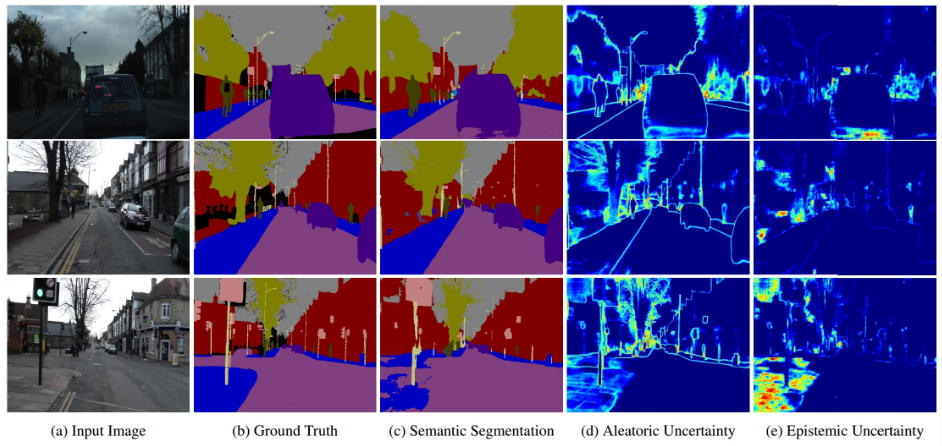
\includegraphics[height=.25\textheight]{Chuong3/Figs/uncertainty.png}
		\label{fig:minh hoa uncertainty}
		\caption{Một ví dụ của uncertainty trong bài toán Semamtation}
	\end{center}
\end{figure}





\begin{spacing}{0.9}
	
	% To use the conventional natbib style referencing
	% Bibliography style previews: http://nodonn.tipido.net/bibstyle.php
	% Reference styles: http://sites.stat.psu.edu/~surajit/present/bib.htm
	
	\bibliographystyle{apalike}
	%\bibliographystyle{unsrt} % Use for unsorted references  
	\bibliographystyle{plainnat} % use this to have URLs listed in References
	\cleardoublepage
	\bibliography{Reference/references} % Path to your References.bib file
	
	
	% If you would like to use BibLaTeX for your references, pass `custombib' as
	% an option in the document class. The location of 'reference.bib' should be
	% specified in the preamble.tex file in the custombib section.
	% Comment out the lines related to natbib above and uncomment the following line.
	
	%\printbibliography[heading=bibintoc, title={References}]
	
	
\end{spacing}
\end{document}